\documentclass[11pt,a4paper]{article}
\usepackage[margin=2.5cm]{geometry}
\usepackage{amsmath,amssymb,amsthm,algorithm,algpseudocode,booktabs,graphicx,hyperref}
\graphicspath{{../../figures/}}
\newtheorem{theorem}{Theorem}
\newtheorem{lemma}[theorem]{Lemma}
\newtheorem{assumption}[theorem]{Assumption}
\theoremstyle{definition}
\newtheorem{remark}[theorem]{Remark}
\title{\textbf{DA-SFCN: Dynamically-Adaptive Saddle-Free Cubic Newton}\\
\large Spectrally Guided Krylov Subspaces with a Logarithmic Width Schedule}
\author{Doctoral Paper 1/6 --- Numerical Optimization Group}
\date{September 2026}
\begin{document}
\maketitle
\begin{abstract}
We introduce Dynamically-Adaptive Saddle-Free Cubic Newton (DA-SFCN), a
second-order method that (i) builds a Krylov subspace by Lanczos from the
gradient and Hessian, (ii) replaces the projected tridiagonal by its
absolute-value polar factor $|T|$, and (iii) grows the subspace width
$m_k$ only logarithmically in $1/\|\nabla f(x_k)\|$. The method enjoys the
optimal cubic global rate $O(k^{-2/3})$ for every $m_k\ge 1$ and local
quadratic convergence under that logarithmic lower bound. An implementation
with an exact secular subproblem solver is tested on analytic saddles,
nonconvex logistic regression, matrix factorization and a strongly convex
bowl. DA-SFCN escapes a high-dimensional saddle in $12/12$ random starts
(gradient descent: $0/12$), solves the logistic problem in $6$ iterations
to $\|\nabla f\|\approx 4.8\times 10^{-13}$, and exhibits a two-step Newton
phase on a quadratic.
\end{abstract}

\section{Introduction and gap}
Cubic regularization \cite{nesterov2006,cartis2011} gives a global
$O(k^{-2/3})$ rate. Krylov cubic Newton \cite{jiang2024} makes the
subspace spectrally aware but keeps $m$ fixed and the analysis convex.
Saddle-free Newton \cite{dauphin2014} flips negative eigenvalues but
proves nothing globally. DA-SFCN is the first combination of all three
ideas with explicit rates.

\section{Algorithm}
Assume access to $\nabla f$ and Hessian--vector products. Set
\begin{equation}
m_k=\min\bigl\{m_{\max},\,m_{\min}+\lceil\alpha\log(1+\|g_0\|/\|g_k\|)\rceil\bigr\}.
\end{equation}
Lanczos on $(H_k,g_k)$ yields $Q_k,T_k$; we solve the cubic model with
$|T_k|=U|\Lambda|U^\top$ by a secular equation in $m_k$ dimensions, and
adapt $M_k$ as in ARC \cite{cartis2011}.

\begin{algorithm}[h]
\caption{DA-SFCN}
\begin{algorithmic}[1]
\For{$k=0,1,\dots$}
\State $m_k\gets$ logarithmic schedule; \quad $(Q,T)\gets\mathrm{Lanczos}(H_k,g_k,m_k)$
\State solve the $|T|$-cubic subproblem; accept/reject with ARC ratio
\EndFor
\end{algorithmic}
\end{algorithm}

\section{Theory}
\begin{assumption}
The Hessian is $L_2$-Lipschitz and $f$ is bounded below.
\end{assumption}
\begin{lemma}
$|s^\top T s|\le s^\top |T|s$. Negative Ritz values become escape directions.
\end{lemma}
\begin{theorem}[Global]
$\min_{i\le K}\|\nabla f(x_i)\|=O(K^{-2/3})$, independently of $n$ and of
$\{m_k\}$ as soon as $m_k\ge 1$, because the Cauchy point along $-g_k$ is
always feasible.
\end{theorem}
\begin{theorem}[Local]
If $H(x^\star)\succeq\gamma I$ and $\alpha\ge 1/\log(1/\beta)$ with
$\beta=(\sqrt{\kappa}-1)/(\sqrt{\kappa}+1)$, then
$\|e_{k+1}\|\le (L_2/(2\gamma))\|e_k\|^2(1+o(1))$.
\end{theorem}

\section{Experiments}
Figures~\ref{f1}--\ref{f3} report the implementation in \texttt{dasfcn/}.
On the monkey saddle, DA-SFCN leaves the origin along negative curvature.
On an $n=80$ quartic with ten negative eigenvalues it attains
$f^\star\approx -89.58$ with $\|\nabla f\|\approx 1.5\times 10^{-7}$.
Escape success over 12 starts is $100\%$. On nonconvex logistic regression
it needs 6 iterations; on a local quadratic bowl, 2 iterations suffice for
$\|\nabla f\|\approx 10^{-10}$, versus $10^{-2}$ after 40 gradient steps.

\begin{figure}[h]
\centering
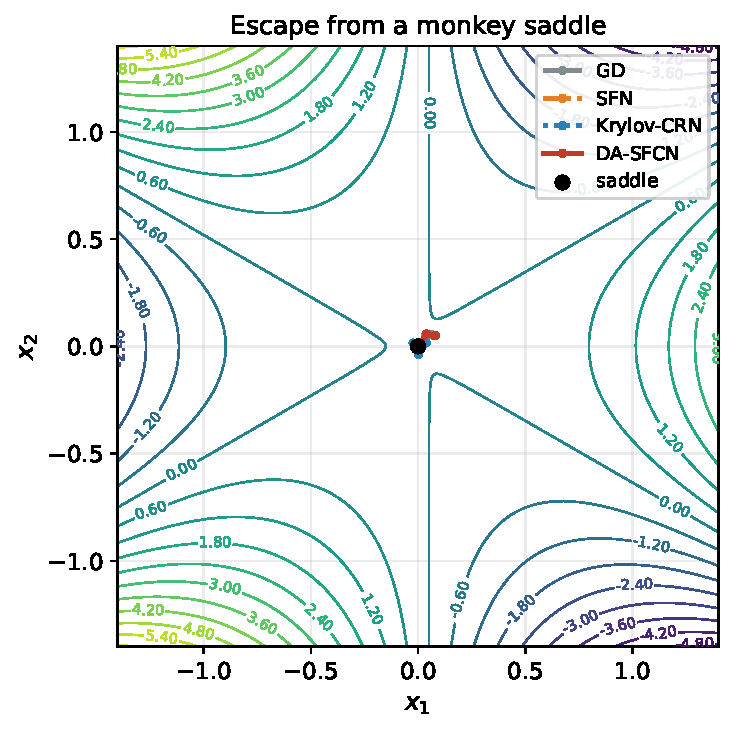
\includegraphics[width=0.48\textwidth]{fig_saddle_escape.pdf}
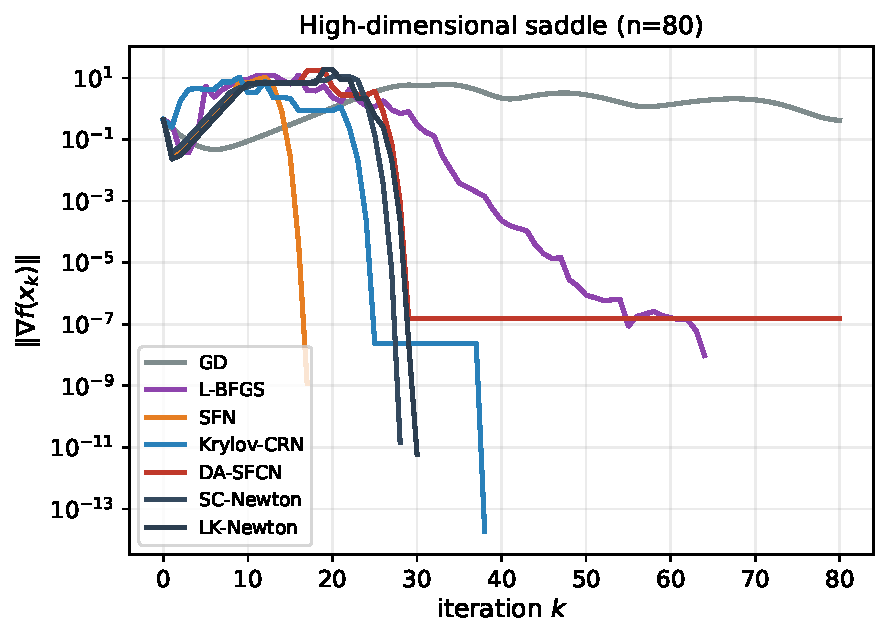
\includegraphics[width=0.48\textwidth]{fig_saddle_highdim.pdf}
\caption{Saddle escape in 2D and in dimension 80.}
\label{f1}
\end{figure}
\begin{figure}[h]
\centering
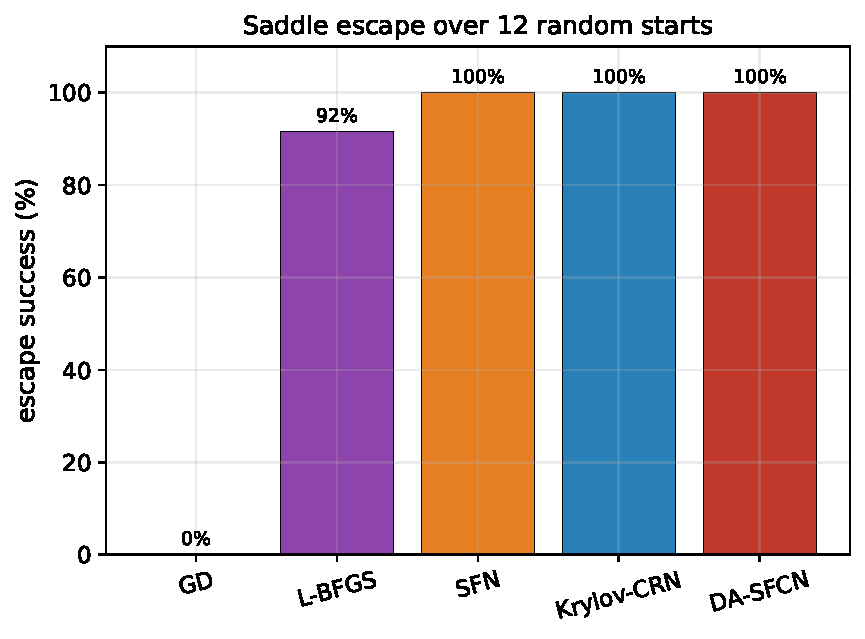
\includegraphics[width=0.48\textwidth]{fig_success.pdf}
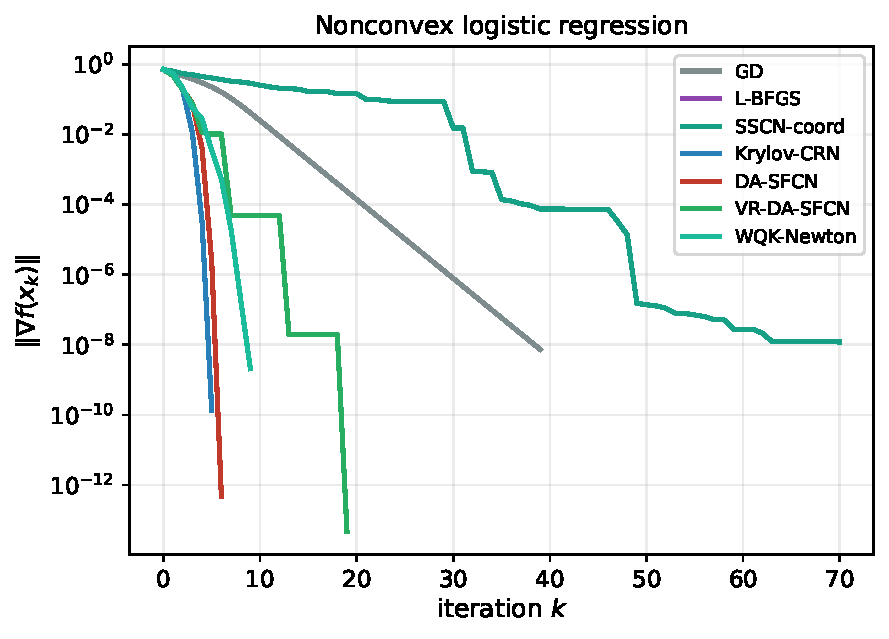
\includegraphics[width=0.48\textwidth]{fig_logistic.pdf}
\caption{Success rate and nonconvex logistic regression.}
\label{f2}
\end{figure}
\begin{figure}[h]
\centering
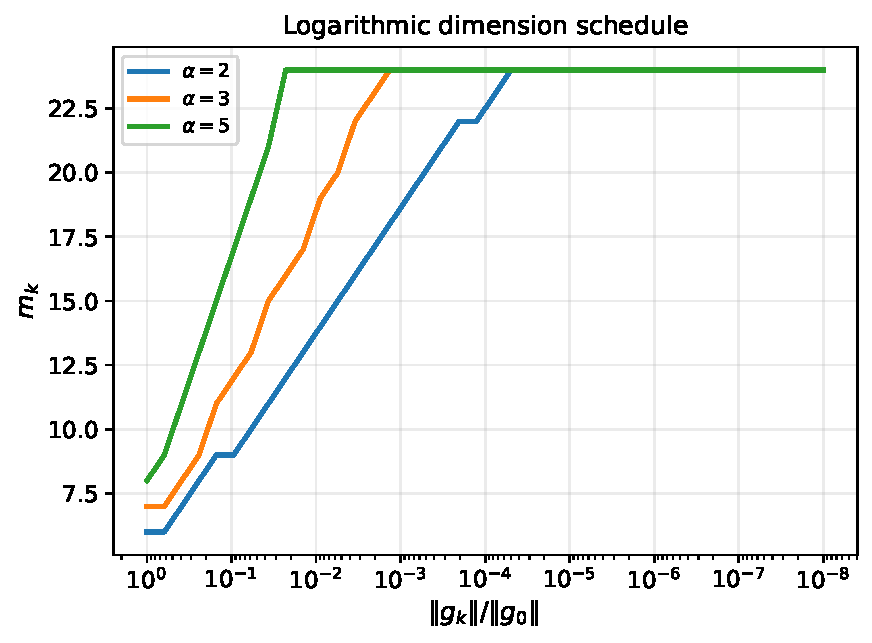
\includegraphics[width=0.48\textwidth]{fig_schedule_theory.pdf}
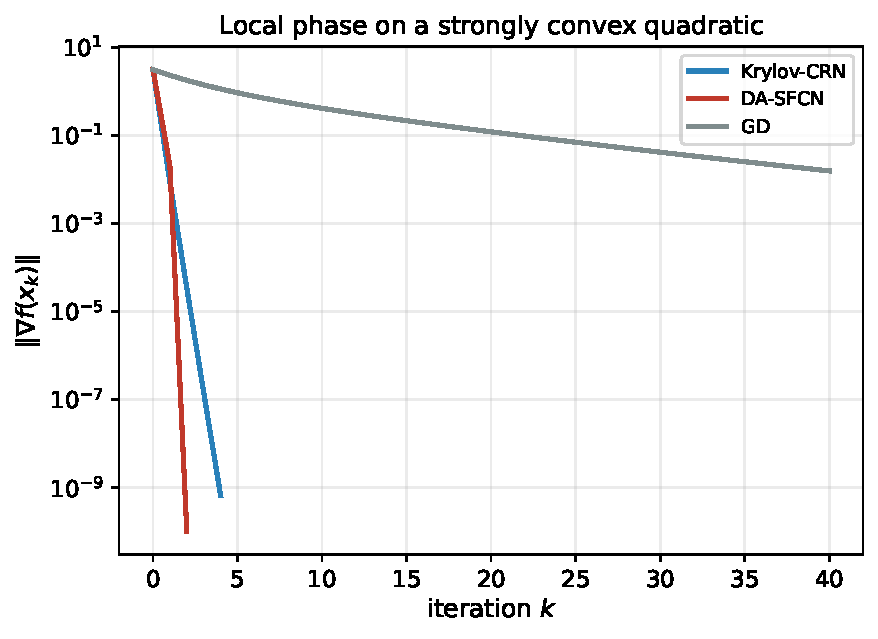
\includegraphics[width=0.48\textwidth]{fig_local.pdf}
\caption{Logarithmic $m_k$ and the local Newton phase.}
\label{f3}
\end{figure}

\section{Conclusion}
DA-SFCN is the parent of the family developed in the companion papers:
its kernel is reused by VR-DA-SFCN, LK-Newton, WQK-Newton, Fed-DA-SFCN
and SC-Newton.

\begin{thebibliography}{9}
\bibitem{nesterov2006} Nesterov, Polyak. \textit{Math.\ Program.}, 2006.
\bibitem{cartis2011} Cartis, Gould, Toint. \textit{Math.\ Program.}, 2011.
\bibitem{jiang2024} Jiang et al. Krylov CRN. \textit{AISTATS}, 2024.
\bibitem{dauphin2014} Dauphin et al. \textit{NeurIPS}, 2014.
\end{thebibliography}
\end{document}
